%_______________________________________________________________________________
%class
%_______________________________________________________________________________
%\documentclass[a4paper,11pt,onecolumn,final,german,openbib]{scrbook}
\documentclass[a4paper,11pt,oneside,final,german,openbib,pdftex]{scrbook}
%_______________________________________________________________________________
% page borders
%_______________________________________________________________________________
\addtolength{\headheight}{2cm}
%\addtolength{\topmargin}{2cm}
\setlength{\oddsidemargin}{1.0cm}
\setlength{\evensidemargin}{0.5cm}
\setlength{\textwidth}{14.3cm}
\setlength{\parindent}{0mm}

%_______________________________________________________________________________
% packages
%_______________________________________________________________________________
\usepackage[english]{babel}
\usepackage{amsmath, amssymb}
\usepackage[utf8]{inputenc}
\usepackage{graphicx}
\usepackage{enumerate}
\usepackage{multirow}
\usepackage{subfigure}
\usepackage{dsfont}
\usepackage{slashed}
\usepackage{textcomp}
\usepackage{url}
\usepackage{amsmath}
\usepackage{hyperref}
\usepackage{tikz}
\usepackage{wrapfig}
\usepackage[backend=bibtex,style=numeric]{biblatex}


\addbibresource{Masterarbeit_Martin_Sobotzik.bib}
%_______________________________________________________________________________
% bold fonts for headings
%_______________________________________________________________________________
\font\afont=cmssbx10 scaled \magstep5     % for the title
\font\bfont=cmssbx10 scaled \magstep4     % for chapter headings
\font\cfont=cmssbx10 scaled \magstep3
\font\dfont=cmssbx10 scaled \magstep2     % for section headings and author name
\font\efont=cmssbx10 scaled \magstephalf

%_______________________________________________________________________________
% index depth
%_______________________________________________________________________________
\setcounter{secnumdepth}{3}
\setcounter{tocdepth}{3}

%_______________________________________________________________________________
% new commands
%_______________________________________________________________________________
\newcommand{\demi}{\frac{1}{2}}

%_______________________________________________________________________________
% renewed commands
%_______________________________________________________________________________
% \renewcommand{\topfraction}{1.}       % this is important for figure placement
% \renewcommand{\bottomfraction}{1.}
\makeatletter
\renewcommand\paragraph{\@startsection{paragraph}{4}{\z@}%
  {-3.25ex\@plus -1ex \@minus -.2ex}%
  {1.5ex \@plus .2ex}%
  {\normalfont\normalsize\bfseries}
}
\makeatother

%_______________________________________________________________________________
% special words, hyphenation
%_______________________________________________________________________________
\hyphenation{Ba-che-lor-ar-beit}

\pagestyle{empty}
\pagestyle{headings}
%for changing the style on a specific page use \thispagestyle{e.g., empty}

%_______________________________________________________________________________
%_______________________________________________________________________________
\begin{document}
\pagenumbering{roman}

%_______________________________________________________________________________
\begin{titlepage}
  \vspace*{6mm}
  \begin{center}
     {\afont Systematic Studies on Reconstruction Efficiency at Belle II}
     \\[3.5cm]
     {\large von}
     \\[3.5cm]
     {\dfont Martin Sobotzik}
     \\[2cm]
     {\large Bachelorarbeit in Physik \/\\
        vorgelegt dem Fachbereich Physik, Mathematik und Informatik (FB 08) \/\\
        der Johannes Gutenberg-Universit\"at Mainz \/\\
        am 3. Dezember 2019}
   \end{center}
   \vfill
   1. Gutachter: Prof. Dr. Wolfgang Gradl\\	
   2. Gutachter: Prof. Dr. Habe D\"unkel \\
   \vfill

\end{titlepage}

\thispagestyle{empty}
Ich versichere, dass ich die Arbeit selbstst\"andig verfasst und keine 
anderen als die angegebenen Quellen und Hilfsmittel benutzt sowie 
Zitate kenntlich gemacht habe.
\\
\\[3.5cm] 
Mainz, den [Datum] [Unterschrift]
\vfill
\noindent 
Martin Sobotzik\\
Institut f\"ur Kernphysik\\
Johannes-Joachim-Becher-Weg 45\\
Johannes Gutenberg-Universit\"at
D-55128 Mainz\\
{\href{msobotzi@students.uni-mainz.de}{msobotzi@students.uni-mainz.de}}

%_______________________________________________________________________________


\renewcommand\contentsname{Contents}
\renewcommand\figurename{Figure}
\renewcommand\tablename{Table}
\tableofcontents
\clearpage

\mainmatter
\sloppy

%_______________________________________________________________________________
\chapter{Introduction}
\label{sec:Introduction}

{\em Dieses Dokument richtet sich an Studierende am Fachbereich 08 im 
Studiengang Bachelor of Science (Physik). Sie finden hier Beispiele 
f\"ur eine m\"ogliche Gliederung Ihrer Arbeit und Hinweise zur 
Strukturierung des Inhalts. Selbstverst\"andlich sollen Sie diese 
Gliederung nach den Gegebenheiten Ihrer Bachelorarbeit anpassen. 
Besprechen Sie rechtzeitig mit Ihrem Betreuer, ob Ihr Entwurf sinnvoll 
ist. Holen Sie sich auch Anregungen zur Gestaltung von Abschlussarbeiten 
aus der Literatur ().
\medskip

Sofern Sie sich dazu entscheiden, Ihr Dokument in \LaTeX\ zu erstellen, 
k\"onnen Sie diese Datei als Vorlage verwenden. Fast die gesamte 
Literatur in der Physik verwendet \LaTeX, vor allem wegen der 
ausgezeichneten M\"oglichkeiten f\"ur das Formelschreiben.
}
\bigskip

In der Einleitung Ihrer Bachelorarbeit sollte das Thema der Arbeit 
m\"oglichst allgemeinverst\"andlich eingef\"uhrt werden. Gehen Sie 
dabei auch auf das weitere Umfeld der Arbeit ein und erl\"autern Sie, 
warum Aufgabenstellung und Herangehensweise interessant sind. Auch 
die weitere Gliederung kann angesprochen werden, um dem Leser einen 
ersten \"Uberblick \"uber den nachfolgenden Text zu geben.

\chapter{Standard Model}







%_______________________________________________________________________________
\chapter{Experimental Setup at SuperKEKB}
\label{sec:SetupKEK}

SuperKEKB is an two-ring, asymmetric\footnote{asymmetric means that there is an energy difference between the two colliding beams}, electron positron accelerator, which is located at KEK (\textit{High Energy Accelerator Research Organization}) in Tsukuba Japan. 
The electron beam has an energy of $7\,\textnormal{GeV}$ 
and the positron beam has an energy of $4\,\textnormal{GeV}$. These beams collide with a center-of-momentum energy of about $10.58\,\textnormal{GeV}$, which is close to the mass of the $\Upsilon(4\textnormal{S})$ resonance. Therefore SuperKEKB is a so called \textit{B-factory}. The decay products are then detected by the  Belle II detector to study the properties of these B mesons with high precision. In early 2018 Belle II started taking data. One goal of Belle II is to study CP-Violation with respect to new physics.\cite{B2B}

\section{KEKB and SuperKEKB}
\label{sec:KEK}
This section will only provide a rough overview of the SuperKEKB accelerator since the focus of this work is on the analysis. 

SuperKEKB is an upgrade of the KEKB accelerator. KEKB was also an asymmetric electron positron accelerator in the period from 1998 to 2010, but the energies were different compared to SuperKEKB. At KEKB the electrons were accelerated to an energy of $8\,\textrm{GeV}$ and the positrons to an energy of $3.5\,\textrm{GeV}$. KEKB was also a B-factory and the reaction products were then detected in the Belle detector. In 2009 KEKB achieved an instantaneous luminosity of $2.11 \cdot 10^{34}\,\textrm{cm}^{-1}\textrm{s}^{-1}$. This was the world record at that time. KEKB was discontinued after more than 10 years, to be upgraded to SuperKEKB.\cite{PTEP}


\begin{figure}[h!]
\begin{center}
	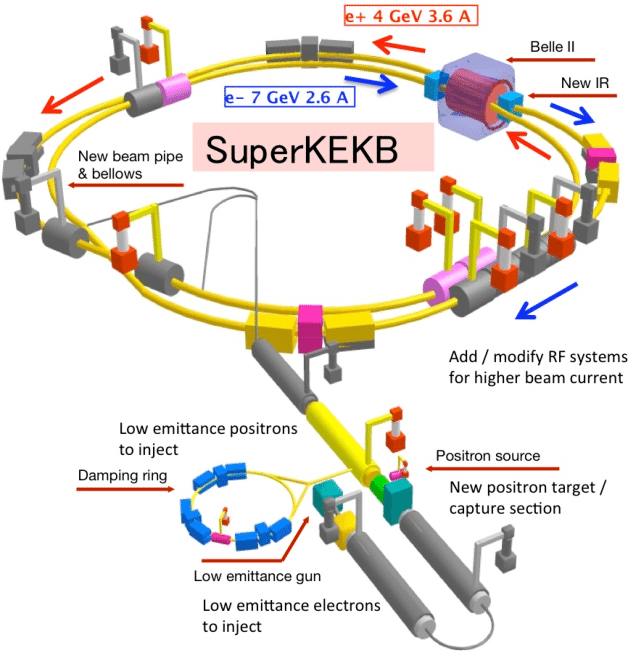
\includegraphics[width=8cm]{Bilder/SuperKEKB.png}
	
	\caption[SuperKEKB Collider]{The SuperKEKB collider.\cite{SKEKAcc}}
	\label{fig:SuperKEKB}
\end{center}
\end{figure}

In figure \ref{fig:SuperKEKB} you can see the schematic layout of the SuperKEKB accelerator. The electrons are start at the Low emittance gun. They are then accelerated in the \textit{J}-shaped linear particle accelerator (linac). Due to lack of space, the linac has to have this special form.\cite{KEKBJArc} After the curve and a second acceleration stage the electrons hit the positron production target, where the positrons are created. After this target there are more acceleration stages, before the two beam are then injected into their independent storage rings. The electrons are stored in the high-energy ring (HER) and the positrons are stored in the low-energy ring (LER). Each of these rings has a circumference of about $3\,\textrm{km}$. Both beams collide at the interaction region (IR). The products of the collisions are then detected by the Belle II detector, an upgraded version of the Belle detector.\cite{B2B} (See chapter \ref{sec:BelleII})

SuperKEKB uses a smaller asymmetry in the beam energies compared to KEKB. This allows the usage for higher beam currents and better focusing magnets. This can then result into a higher luminosity. The goal is to achieve a 40 times higher luminosity with SuperKEKB compared to KEKB.
An integrated luminosity of $50\,\textrm{ab}^{-1}$ will be achieved by 2025.\cite{B2B}

The instantaneous luminosity $\mathcal{L}$ specifies the performance of the collider. Knowing $\mathcal{L} $ and the cross section $\sigma$ one can calculate the events per second for a process by the following formula.
\begin{equation}
\frac{\textrm{d}N}{\textrm{d}t} = \mathcal{L} \cdot \sigma
\end{equation} 

To increase the event rate one has to increase the instantaneous luminosity since $\sigma$ is given by the processes. The instantaneous luminosity can be calculate by
\begin{equation}
	\mathcal{L} = \frac{N_{e^-}N_{e^+}f_c}{4\pi \sigma_x \sigma_y} \cdot S
	\label{eq:Lumi}
\end{equation}
 assuming that both beams have a Gaussian profile of horizontal and vertical size $\sigma_x$ and $\sigma_y$. In equation \ref{eq:Lumi} $N_{e^-}$ is the number of particles in an electron bunch and $N_{e^+}$ is the number of particles in a positron bunch. $f_c$ is the average crossing rate, which can be calculated by $f_c = n \cdot f_r$. Where $n$ is the number of bunches and $f_r$ is the revolution frequency. $S$ is a reduction factor which takes geometrical effects linked to the finite cross section and bunch length into account.\cite{herr2006concept} SuperKEKB increased the luminosity by a factor of two compared to KEKB by increasing the number of bunches and the number of particles per bunch.
 
\begin{figure}[h!]
	\centering
	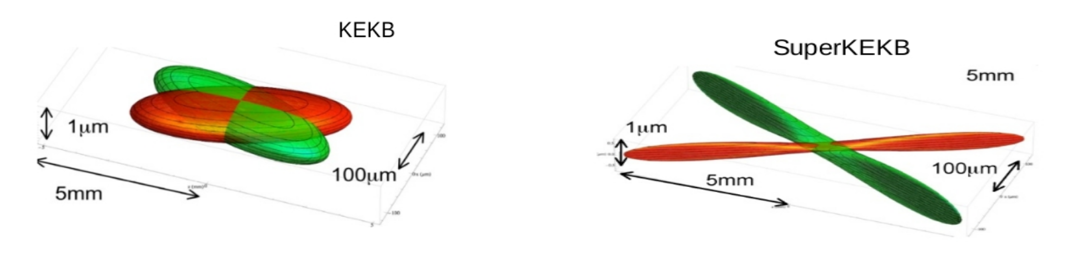
\includegraphics[width=14.5cm]{Bilder/bsSKEK}
	
	\caption[Sketch of the Beam Crossing for KEKB and SuperKEKB]{Sketch of the beam crossing at KEKB (left) and SuperKEKB (right). At KEKB the size of the interaction region was about $10\,\textrm{mm}$. At SuperKEKB it is about $0.5\,\textrm{mm}$}
	\label{fig:beamsize}
\end{figure}

Also the size of the interaction region at SuperKEKB is just one twentieth of what it was at KEKB, resulting in a vertical beam size of $\sigma \approx 50\,\textrm{nm} $. This can be seen in figure \ref{fig:beamsize}. This decrease in beam size, along with the increase in the beam currents, it results in a overall 40-fold increase in luminosity.  \cite{B2TR} \cite{B2B}



\section{The Belle II Detector}
\label{sec:BelleII}

The Belle II detector is an upgraded version of the Belle detector which was a solid-angle magnetic spectrometer located at the interaction region of KEK. In figure  \ref{fig:Belle2} a sketch of the Belle II detector is shown. The detector contains of a variety of sub-detectors, each fulfilling a specific purpose.
 
\begin{figure}[h!]
	\centering
	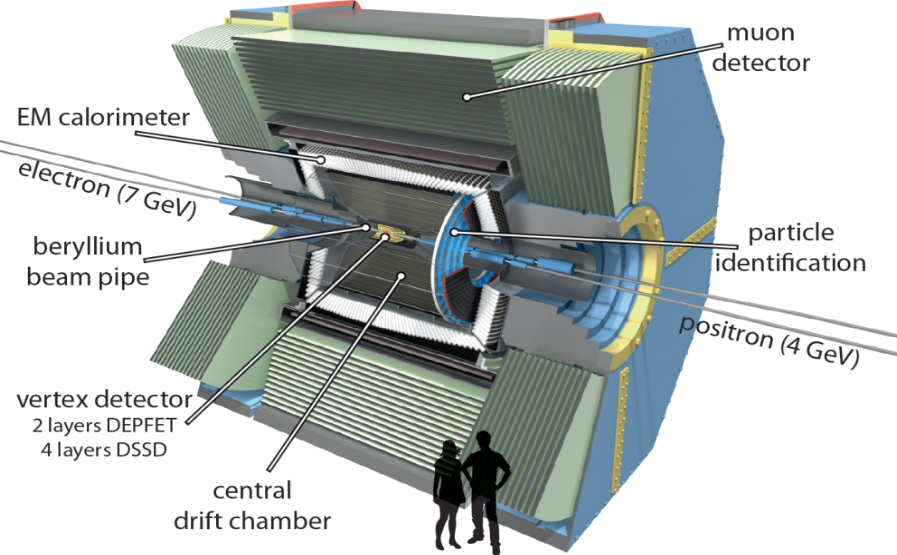
\includegraphics[width=14.5cm]{Bilder/Belle2.png}
	
	\caption[Belle II Detector]{Schematic view of the Belle II detector. The different detector elements are labeled. Also the beam pipes for the electrons and positrons with their corresponding energies are shown. \cite{BDetector}}
	\label{fig:Belle2}
\end{figure}

 In the innermost of the detector, three tracking sub-detectors are located, surrounding the IR. These sub-detectors are in a axial magnetic field of $1.5\,\textrm{T}$, provided by a solenoid, to be able to reconstruct the tracks of charged particles. 
 
 The vertex detectors, consisting of the silicon vertex detector (SVD), an upgraded version of the SVD used in Belle, and the pixel detector (PXD), a new detector designed for Belle II, are used to measure the momenta of charged particles and to reconstruct decay vertices and particles with a momentum to low to reach the central drift chamber (CDC).

The CDC also already existed in the Belle detector and has been upgraded for Belle II. The CDC scans the trajectories of charged particles. From these trajectories the charge, momentum and energy loss can be determined by ionization. 

These three innermost tracking detectors are surrounded by a barrel. The time-of-propagation (TOP) detector, which also got an upgrade for Belle II, surrounds the inner detectors parallel to the beam-pipes. The TOP detector, as the name suggests, measures the flight-time of charged particles. Knowing the flight-time and the momentum of the charged particles, it is possible to conclude their mass and to identify them. In the forward end-cap of the barrel are closed with an Aerogel Ring-Imaging Cherenkov detector (ARICH) which also identifies charged particles.

The next outer detector is the electromagnetic calorimeter (ECL). It surrounds all the previously mentioned detectors, and was already installed in Belle. With the ECL the energy of electromagnetically interacting particles, especially photons and electrons, can be measured.

The task of the outermost detector the $K_L^0$ and muon detector (KLM) is to identify $K_L^0$ and muons. The KLM also got upgraded for Belle II. \cite{B2B} 

\section{Coordinate System}

For clarification, I want to explain the coordinate system of Belle II, before I describe to the detectors in more detail.

\begin{figure}[h!]
	\begin{center}
		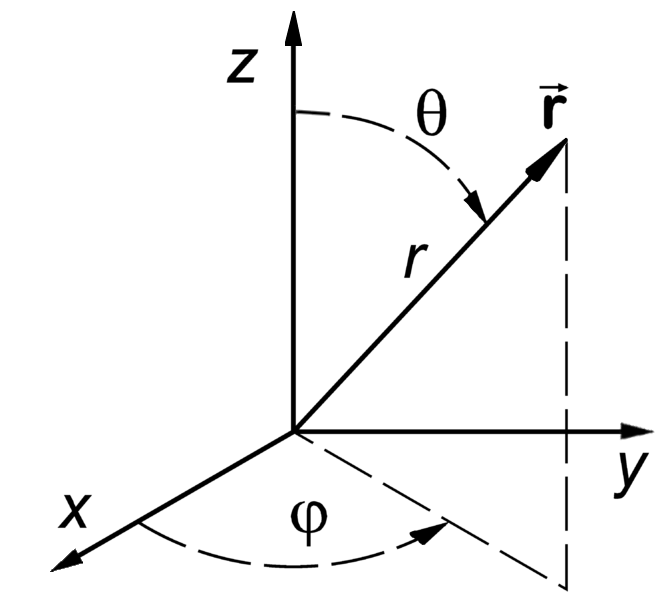
\includegraphics[width=4.5cm]{Bilder/coordinate.png}
	\end{center}
	\caption[Coordinate System of Belle II]{A sketch of the coordinate system of Belle II}
	\label{fig:CoordinateSysytem}
\end{figure}

A sketch of the coordinate system is shown in figure \ref{fig:CoordinateSysytem}. The origin of the coordinate system corresponds to the interaction region. For the Cartesian coordinate system: The $z$-axis points in the direction of the magnetic field. This is also the so called forward direction. The $y$-axis points up to the upper part of the detector. The $x$-axis points along the radial direction of the accelerator. In figure \ref{fig:CoordinateSysytem} also the spherical coordinate system is shown. Here $\theta$ corresponds to the polar angle and $\phi$ to the azimuthal angle.\cite{DevelopVertex}

\section{Vertex detector}
\label{sec:vertexDet}

The vertex detectors (VXD) is able to make precise measurements of the tracks of particles close to the interaction region. This allows the reconstruction of decay-vertices of long-lived particles. For this it is very important to determine the distance and the spatial resolution of the first measured hit, and the effect of multiple scattering.


\begin{figure}[h!]
	\begin{center}
		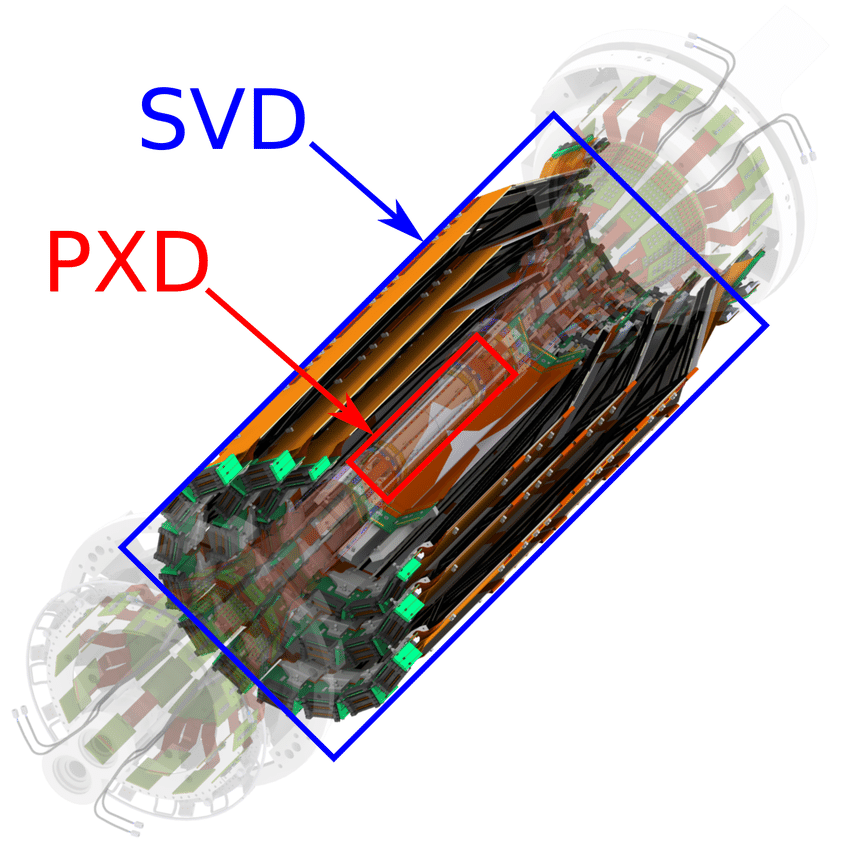
\includegraphics[width=10.5cm]{Bilder/PXD_SVD}
	\end{center}
\caption[Vertex Detector]{Sketch of the vertex detectors. The vertex detector itself consists of two sub-detectors. The PXD is surrounded by the SVD. \cite{OnlineDataReduction} }
\label{fig:VertexDet}
\end{figure}

The VXD consists of the pixel vertex detector and the silicon vertex detector, both can be seen in figure \ref{fig:VertexDet}. These two detectors complement each other.


\subsection{Pixel Vertex Detector}
\label{sec:Pixel}
The purpose of the PXD is to reconstruct the spatial position of the decay vertices of $B$, $D$ and $\tau$.
The PXD is based on Depleted P-channel Field-Effect Transistor (DePFET) technology. This technology allows the sensors of the PXD to be very thin ($50\,\mu\textrm{m}$).

\begin{figure}[h!]
	\begin{center}
		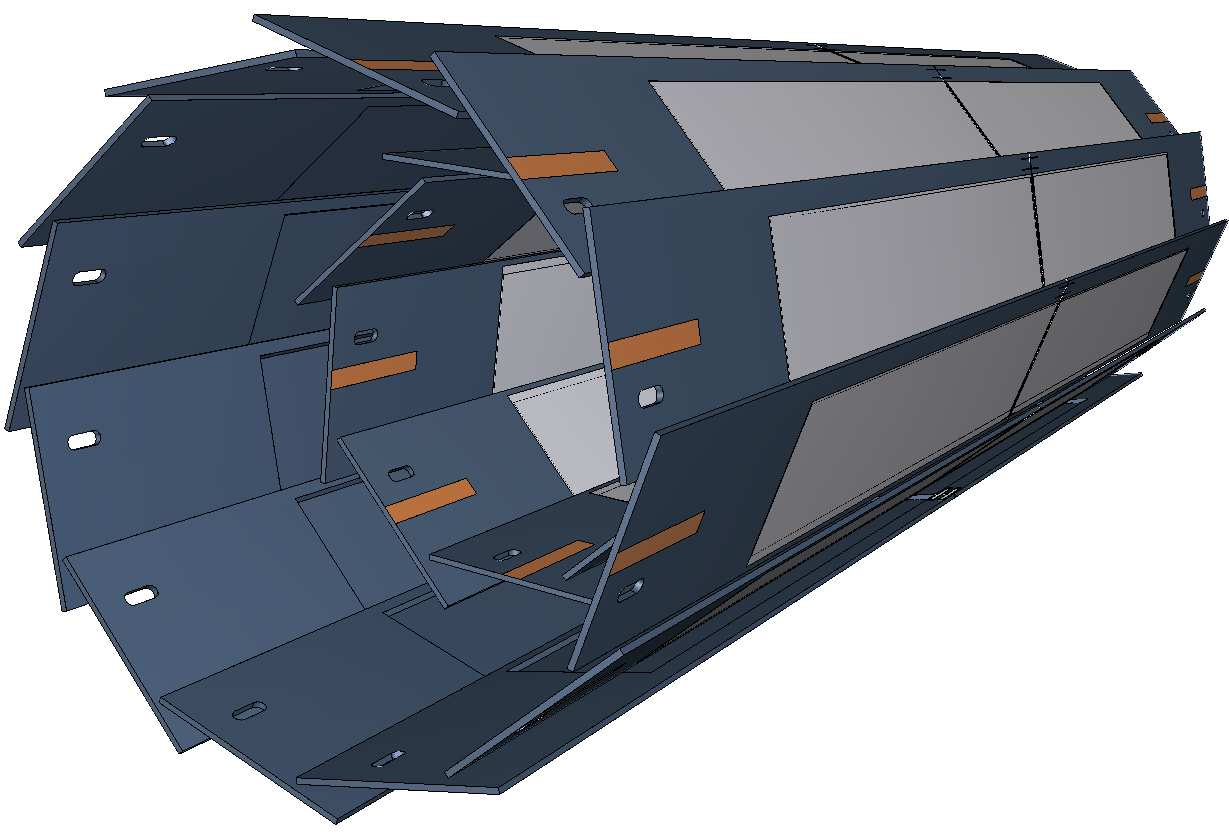
\includegraphics[width=10.5cm]{Bilder/pixel}
	\end{center}
	\caption[Pixel Detector]{Sketch of the PXD \cite{B2TR}}
	\label{fig:pxd}
\end{figure}

As you can see in figure \ref{fig:pxd}, the PXD consists of two layers of sensors. The inner layer is made out of eight planar sensors (ladder), each has a width of $15\,\textrm{mm}$ and an effective length of $90\,\textrm{mm}$. This layer has a radius of $14\,\textrm{mm}$. The second layer consists of 12 planar sensors. These sensors also have a width of $15\,\textrm{mm}$, but a length of $123\,\textrm{mm}$. The radius for the second layer is $22\,\textrm{mm}$. 

Due to the vicinity of the PXD to the interaction region, the quantum-electrodynamics background is very high, so the sensors  must withstand high radiation. The DePFET technology fulfills this condition. \cite{B2TR}

DePFET

\begin{figure}[h!]
	\begin{center}
		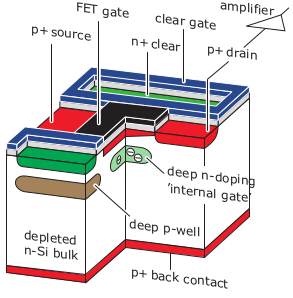
\includegraphics[width=7cm]{Bilder/DEPFET}
	\end{center}
\caption[DePFET]{Illustration of the DePFET technology.\cite{B2TR}}
\label{fig:DePFET}
\end{figure}


\subsection{Silicon Vertex Detector}
\label{sec:Silicon}

%_______________________________________________________________________________
\section{Grundlagen}

Beschreiben Sie bei einer experimentellen Arbeit die wesentlichen 
theoretischen Grundlagen und in jedem Fall den Stand der Forschung.

\section{Versuchsaufbau}

Wenn Sie an einem experimentellen Thema arbeiten, beschreiben Sie 
den Versuchsaufbau, auch wenn Sie an einem bereits vorhandenen 
Versuch arbeiten, soweit dies f\"ur Ihre spezielle Fragestellung 
relevant ist. 


\chapter{BASF2}
\label{BASF2}


\section{Methoden}

Entsprechend kann es bei einer theoretischen Arbeit sinnvoll sein,
die L\"osungsmethoden in einem eigenen Kapitel zu beschreiben.

\section{Ergebnisse}

Hauptteil Ihrer Arbeit ist das Kapitel (oder die Kapitel) mit den 
Ergebnissen. Bei einer theoretischen Arbeit kann damit auch 
die Herleitung von Formeln oder die Beschreibung eines Computerprogramms 
gemeint sein.

%_______________________________________________________________________________
\chapter{Zusammenfassung und Ausblick}

In der Zusammenfassung sollten Sie in knapper Form die Aufgabenstellung 
und die wichtigsten Ergebnisse rekapitulieren. Es ist f\"ur die 
Gutachter hilfreich, wenn Sie ausdr\"ucklich beschreiben, worin 
Ihre eigenen Beitr\"age liegen. Scheuen Sie sich auch nicht davor 
auszusprechen, welche Untersuchungen durch die Zeitbegrenzung der 
Bachelorarbeit nicht m\"oglich waren und nutzen Sie dies als 
\"Uberleitung zu einem Ausblick auf m\"ogliche weitergehende 
Arbeiten an der Aufgabenstellung.

%_______________________________________________________________________________
\begin{appendix}
\chapter{Appendix}

\section{Tabellen und Abbildungen}

In der Regel sind die in Tabellen und Abbildungen enthalten Informationen 
so wichtig, dass sie im Hauptteil der Arbeit erscheinen sollten. Unter 
Umst\"anden sind aber erg\"anzende Tabellen und Abbildungen gut in einem 
Anhang aufgehoben. Wie im Hauptteil sollten Sie auch hier darauf achten, 
dass die in Tabellen und Figuren (siehe Abb.\ \ref{Abb:1}) dargestellte 
Information im Text angesprochen wird und selbsterkl\"arende Legenden 
vorhanden sind.
\medskip


%_______________________________________________________________________________
\section{Weiterf\"uhrende Details zur Arbeit}

Manch wichtiger Teil Ihrer tats\"achlichen Arbeit ist zu technisch 
und w\"urde den Hauptteil des Textes un\"ubersichtlich machen, 
beispielsweise wenn es um die Details des Versuchsaufbaus in einer 
experimentellen Arbeit oder um den f\"ur eine numerische Auswertung 
verwendeten Algorithmus geht. Dennoch ist es sinnvoll, entsprechende 
Beschreibungen in einem Anhang Ihrer Bachelorarbeit aufzunehmen. 
Insbesondere f\"ur zuk\"unftige Arbeiten, die an Ihre Bachelorarbeit 
anschlie{\ss}en, sind dies manchmal hilfreiche Informationen.

%_______________________________________________________________________________
\listoffigures
\listoftables
%\chapter{Bibliography}

Machen Sie genaue Angaben, so dass die verwendeten Literaturstellen 
eindeutig identifiziert und aufgefunden werden k\"onnen.
Bei Lehrb\"uchern ist es sinnvoll, 
den Titel anzugeben, eventuell auch die Ausgabe. Bei Artikeln in 
Fachzeitschriften ist es \"ublich, nur die 
gebr\"auchlichen Abk\"urzungen f\"ur den Titel der Zeitschrift, Band, 
Erscheinungsjahr und Seite anzugeben. Unter Umst\"anden kann es auch 
sinnvoll sein, im Internet aufgefundene Informationsquellen anzugeben, 
zum Beispiel f\"ur Software oder zu den Details von 
Ergebnissen gro{\ss}er experimenteller Kollaborationen. Es ist 
selbstverst\"andlich, dass Sie auch Bachelor, 
Diplom- oder Doktorarbeiten angeben, wenn Sie diese in Ihrer eigenen 
Arbeit verwendet haben.
\medskip

Im folgenden Beispiel werden die in der Datei %{\tt h-physrev3.bst} 
enthaltenen Anweisungen als Stilvorlage verwendet. Andere 
M\"oglichkeiten f\"ur die Gestaltung eines Literaturverzeichnisses 
findet man im Internet: \url{http://janeden.net/bibliographien-mit-latex}.


\nocite{*}
\printbibliography



%_______________________________________________________________________________
\chapter{Danksagung}

... an wen auch immer. Denken Sie an Ihre Freundinnen und Freunde, 
Familie, Lehrer, Berater und Kollegen.

\end{appendix}

\end{document}  
        
        